\documentclass[12pt, a4paper, oneside, titlepage]{article}
\usepackage{geometry}
\usepackage{fancyhdr}
\usepackage{amsmath, amsthm, amssymb}
\usepackage{graphicx}
\usepackage{hyperref}
\usepackage{array}
\usepackage[english]{babel}
\usepackage[table]{xcolor}
\usepackage{rotating}
\usepackage{multirow}
\usepackage{supertabular}
\usepackage{subfig}

\newcommand{\HRule}{\rule{\linewidth}{0.5mm}}

\pagestyle{fancy}
\fancyhf{}


\fancyhead[RO] {\thepage}
%\fancyhead[LO]{\rightmark}
%\fancyhead[RE]{\leftmark}
%\fancyhead[RE]{\textit{\nouppercase{\leftmark}}}
\fancyhead[LO]{\textit{\nouppercase{\rightmark}}}


\fancypagestyle{plain}{ %
\fancyhf{} % remove everything
\renewcommand{\headrulewidth}{0pt} % remove lines as well
\renewcommand{\footrulewidth}{0pt}}

\begin{document}

\begin{titlepage}
\begin{center}
\thispagestyle{empty}

\textsc{\large Norwegian University of Science and Technology} \\
\textsc{IT3708 - Subsymbolic Methods in AI} \\[3cm]
%\textsc{Group 13} \\[3cm]
\HRule\\[0.5cm]
{\Huge Evolving Spiking-Neuron Parameters}\\[0.5cm]
%\textsc{\large Colonel Blotto}
\HRule\\[5.5cm]

{\large \emph{Author:}}\\
Jonas Eikli\\
Erlend B\o rslid Haugsdal

\vfill

{\large \today}


\end{center}
\end{titlepage}




\addcontentsline{toc}{section}{Contents}
\tableofcontents

\newpage
\section{Description}
To solve this problem we have added two new classes to our project, SpikingNeuronPhenotype and SpikeTrainDistanceMetrics. 
SpikingNeuronPhenotype is our phenotype representation of the problem. The genotype is a 50 size bitset. Each 10 bit represent a parameter giving 1024 different values for mutation and crossover.
The phenotype read this bitset and creates a spike train based on the values with 1001 timesteps. 

The FitnessTesting class takes evaluationMethod and trainingDataset as new integer parameters and has a new subclass, the SpikeTrainDistanceMetrics. When the SpikeTrainDistanceMetrics is initiated it reads the target data from file and creates a target spike train and target spike position array. A class diagram can be seen in Figure \ref{classdiagram}

\begin{figure}
	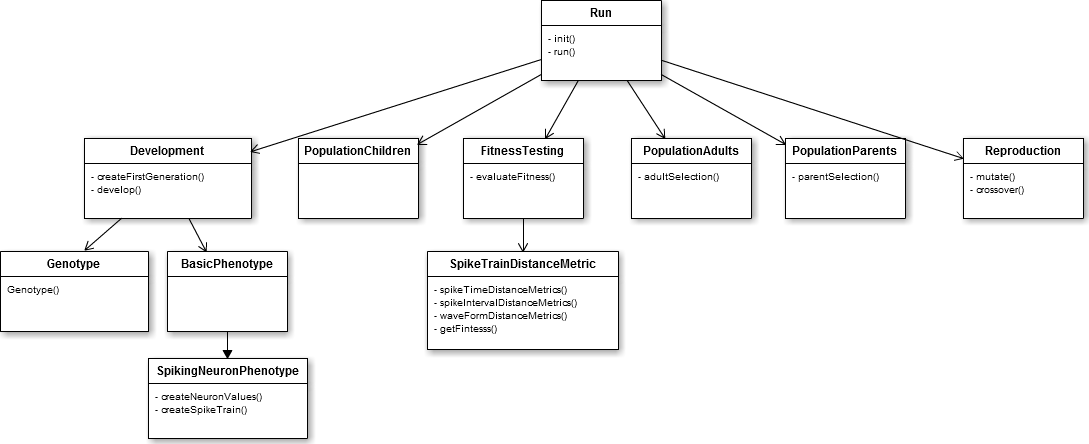
\includegraphics[width=\textwidth]{klassediagram}
	\caption{A class diagram}
	\label{classdiagram}
\end{figure}
For each generation and phenotype the class then calculate the distance between the neuron and target train. The fitness is calculated with 1/(distance+1). This gives a fitness value between 0 and 1, as the optimal distance is 0.

For adult selection we used a combination of the methodes implemented in exercise 1. It used generation mixing 70\% of the time and over production the rest of the time. This way we allow a full generation change from time to time as this allow some new phenotypes a chance to grow up. 

For parent selection er used sigma scaling, this proved to give the best results. We used a generation pool of 200 and 40 adults. Crossover is random over the entire bitset and mutation is 5\%.  


\section{Analysis}

The results from the 12 test runs can be seen in Figure \ref{spiketime}, \ref{spikeinterval} and \ref{wave}. Their respective fitness progression can be seen in Figure \ref{spiketimefitness}, \ref{spikeintervalfitness} and \ref{wavefitness}. The fitness graphs shows in what generation there was an improvement to the fitness.

Figure \ref{spiketime} shows all the different test cases made with the Spike Time Distance Metrics. Likewise, Figure \ref{spikeinterval} shows the ones made with Spike Interval Distance Metrics and Figure \ref{wave} shows the ones with Waveform Distance Metrics. 

Table \ref{table} shows the fitness value and the parameters used to make each of the spike trains in the figures.

\subsection{Description of the Test Runs}
\begin{description}
\item[Test Run 1] \hfill \\
	This test run is shown in Figure \ref{activation1}. This was a very good result, as the test run looks a lot like the target spike train. The best result for the first target spike train.
\item[Test Run 2] \hfill \\
	This test run is shown in Figure \ref{activation4}. Another good result. The best for the second target spike train. It must be noted that the height of the peaks does not match the target spike trains in any of the runs, but this is because the target spike trains is capped at 35, while the test runs is not.
\item[Test Run 3] \hfill \\
	This test run is shown in Figure \ref{activation7}. Yet another good result.
\item[Test Run 4] \hfill \\
	This test run is shown in Figure \ref{activation10}. This one did not score very well, however, it must be said that it is quite similar to the target spike train. All in all, the Spike Time Distance Metrics performed really well, as all the test runs ended up looking good.
\item[Test Run 5] \hfill \\
	This test run is shown in Figure \ref{activation2}. This was one of the least similar test runs. Also the one with the lowest fitness. 
\item[Test Run 6] \hfill \\
	This test run is shown in Figure \ref{activation5}. This was a quite good test run, and ended up looking really good.
\item[Test Run 7] \hfill \\
	This test run is shown in Figure \ref{activation8}.	A fairly good test run.
\item[Test Run 8] \hfill \\
	This test run is shown in Figure \ref{activation11}. This test run got a really good fitness value (0.84), but it does not look that much like the target spike train.
\item[Test Run 9] \hfill \\
	This test run is shown in Figure \ref{activation3}. Does not look like the target test run. The peaks are in approximately the right position, but there are not enough of them.
\item[Test Run 10] \hfill \\
	This test run is shown in Figure \ref{activation6}. This test run look nothing like the target spike train, but it got a fitness value of 0.83. The waveform distance metrics did not work very well on this target.
\item[Test Run 11] \hfill \\
	This test run is shown in Figure \ref{activation9}. A very good test run. Got the highest fitness value (0,86). The best for the third target spike train.
\item[Test Run 12] \hfill \\
	This test run is shown in Figure \ref{activation12}. This is the closest to the fourth target spike train. Very good.
\end{description}

\begin{table}
	\begin{tabular}{|l|l|l|l|l|l|l|} 
	\hline
	Spike Train & Best fitness & A & B& C& D& K \\ \hline
	Figure \ref{activation1} & 0,74 & 	 0.02609& 0.08030&-48.76832& 1.85161	&0.04096\\
	Figure \ref{activation4} & 0,52	&    0.00100& 0.03636&-78.82697& 8.54838	&0.05645\\
	Figure \ref{activation7} & 0,78&	 0.10721& 0.10411& -49.89247&	 3.10967& 0.0400\\
	Figure \ref{activation10} & 0,40&  	 0.02356& 0.27930& -48.03519& 5.49032&	 0.04677\\ \hline
	Figure \ref{activation2} & 0,40&  	 0.03504& 0.09787& -45.59139&	 6.32258&	 0.04774\\
	Figure \ref{activation5} & 0,67&	 0.00138& 0.03608&	 -75.99217&	 8.61612&	 0.060322\\
	Figure \ref{activation8} & 0,55&	 0.06908& 0.16478& -36.15835&	 6.74838& 0.04000\\
	Figure \ref{activation11} & 0,84&	 0.031346& 0.23735&	 -40.70381&	 4.28064&	 0.040967\\ \hline
	Figure \ref{activation3} & 0,70&	 0.101569& 0.12991&	 -37.38025&	 7.68709&	 0.04000\\
	Figure \ref{activation6} & 0,83&	 0.003139& 0.15259& -57.90811&	 9.95161& 0.07967\\
	Figure \ref{activation9} & 0,86&	 0.003334& 0.01028& -45.24926&	 6.39999& 0.06032\\
	Figure \ref{activation12} &0,80&	 0.003139& 0.12424& -53.90029&	 9.51612& 0.07677\\ \hline
	\end{tabular}
	\caption{The fitness value for, and the parameters used to make, the closest-to-target spike train for each of the 12 test-runs. Note: the values have been rounded off to fit in the table.}
	\label{table}
\end{table}


\begin{figure}
	\centering
	\subfloat[Spike train 1]{\label{activation1}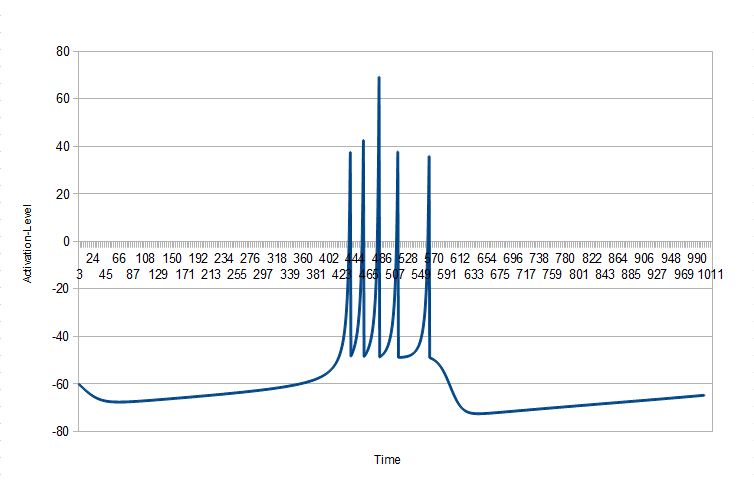
\includegraphics[width=0.5\textwidth]{graphs/activationlevel1}}
	\subfloat[Spike train 2]{\label{activation4}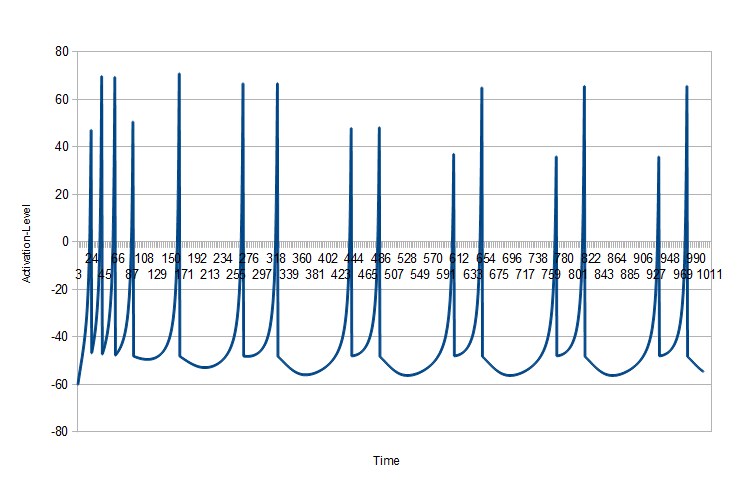
\includegraphics[width=0.5\textwidth]{graphs/activationlevel4}}\\
	\subfloat[Spike train 3]{\label{activation7}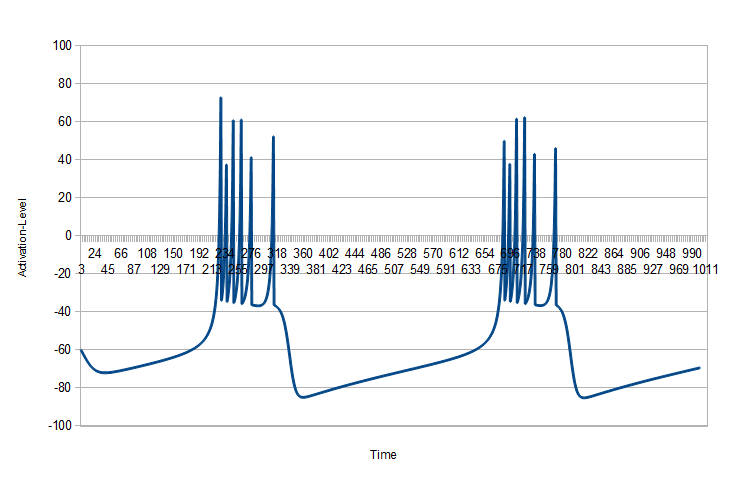
\includegraphics[width=0.5\textwidth]{graphs/activationlevel7}}
	\subfloat[Spike train 4]{\label{activation10}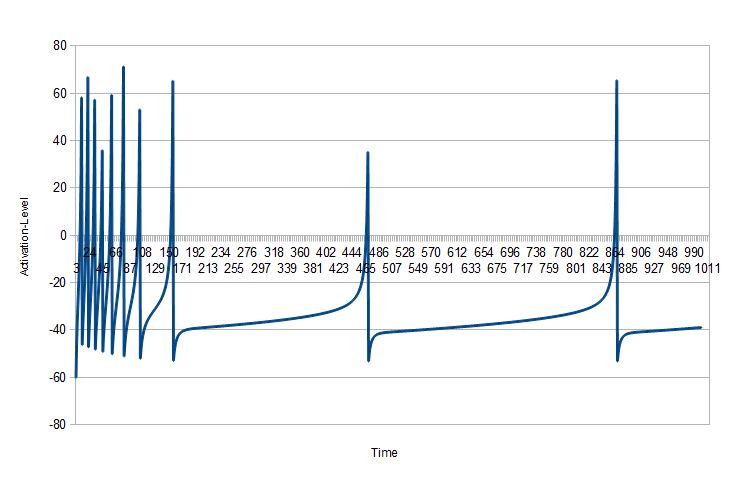
\includegraphics[width=0.5\textwidth]{graphs/activationlevel10}}
	\caption{This is the closest-to-target spike trains developed with Spike Time Distance Metrics.}
	\label{spiketime}
\end{figure}

\begin{figure}
	\centering
	\subfloat[Spike train 1]{\label{fitness1}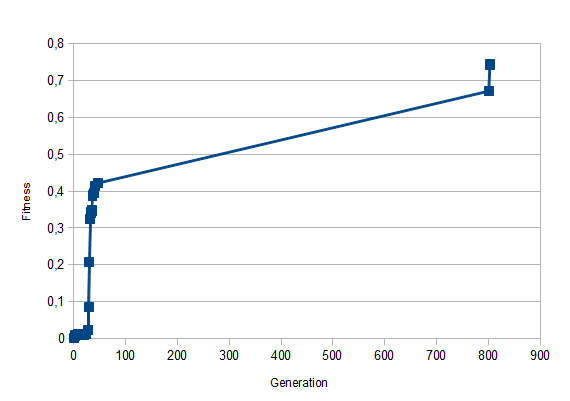
\includegraphics[width=0.5\textwidth]{graphs/fitness1}}
	\subfloat[Spike train 2]{\label{fitness4}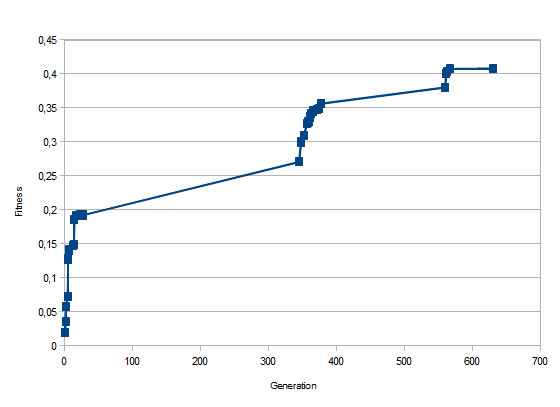
\includegraphics[width=0.5\textwidth]{graphs/fitness4}}\\
	\subfloat[Spike train 3]{\label{fitness7}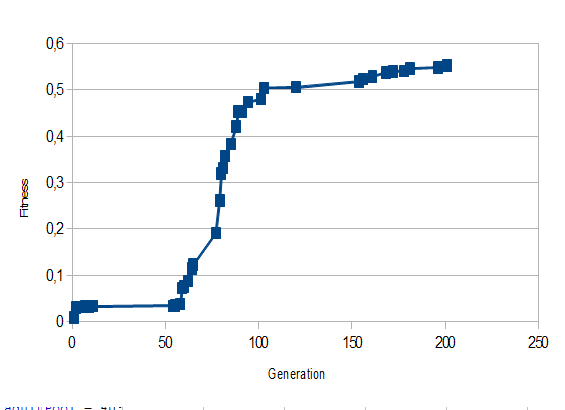
\includegraphics[width=0.5\textwidth]{graphs/fitness7}}
	\subfloat[Spike train 4]{\label{fitness10}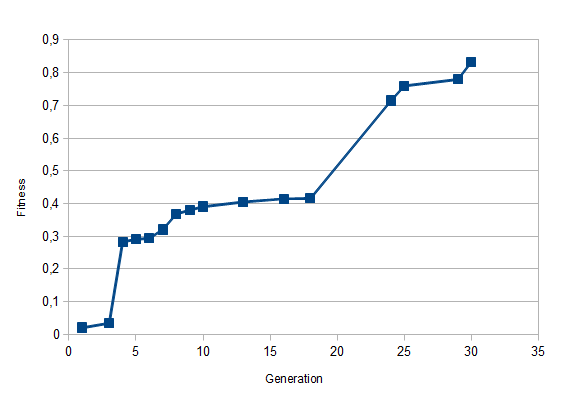
\includegraphics[width=0.5\textwidth]{graphs/fitness10}}
	\caption{This is the fitness graph matching the spike trains developed with Spike Time Distance Metrics.}
	\label{spiketimefitness}
\end{figure}




\begin{figure}
	\centering
	\subfloat[Spike train 1]{\label{activation2}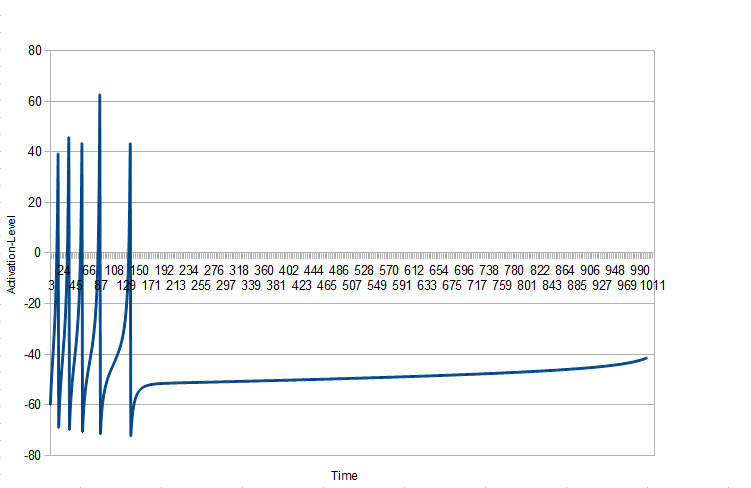
\includegraphics[width=0.5\textwidth]{graphs/activationlevel2}}
	\subfloat[Spike train 2]{\label{activation5}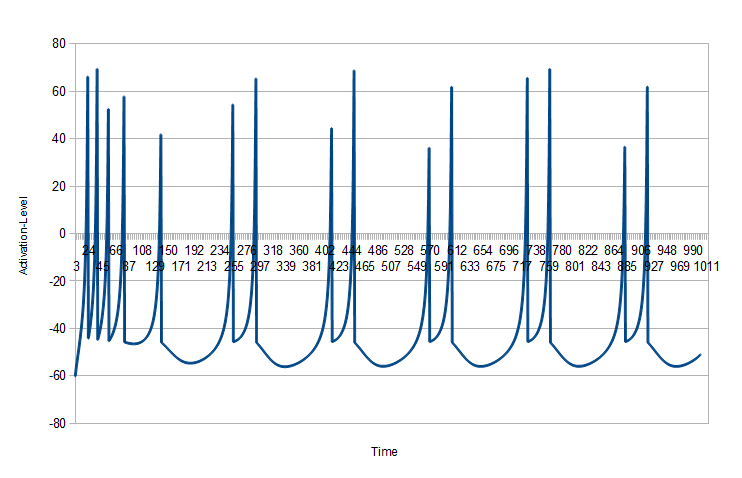
\includegraphics[width=0.5\textwidth]{graphs/activationlevel5}}\\
	\subfloat[Spike train 3]{\label{activation8}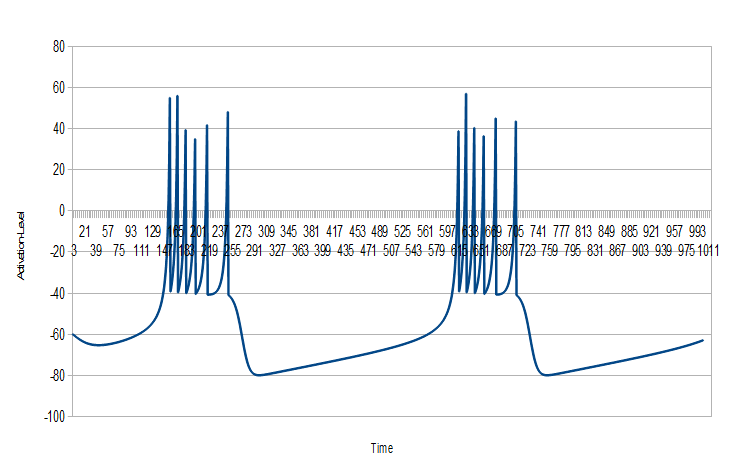
\includegraphics[width=0.5\textwidth]{graphs/activationlevel8}}
	\subfloat[Spike train 4]{\label{activation11}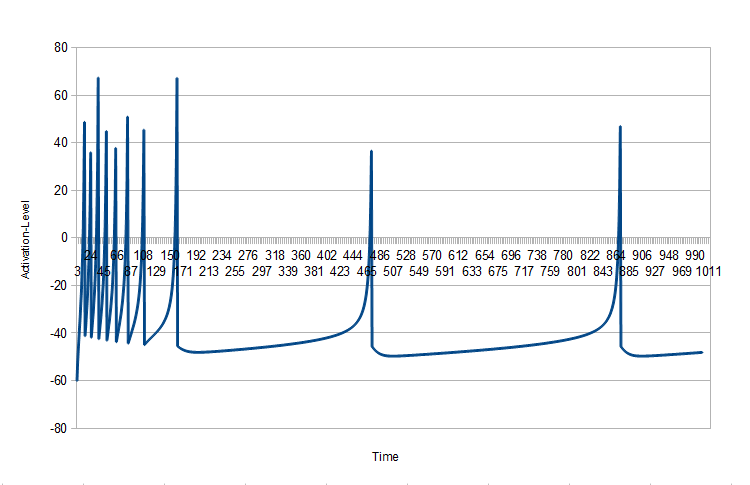
\includegraphics[width=0.5\textwidth]{graphs/activationlevel11}}
	\caption{This is the closest-to-target spike trains developed with Spike Interval Distance Metrics.}
	\label{spikeinterval}
\end{figure}

\begin{figure}
	\centering
	\subfloat[Spike train 1]{\label{fitness2}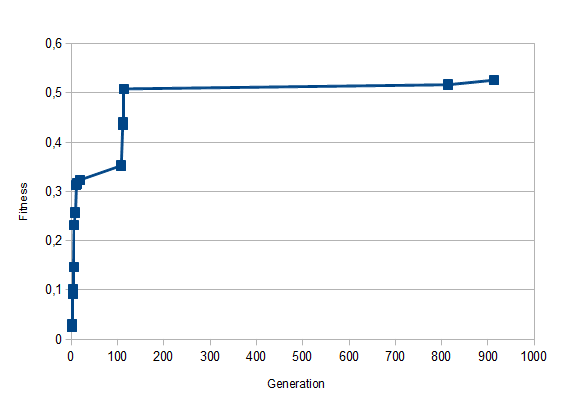
\includegraphics[width=0.5\textwidth]{graphs/fitness2}}
	\subfloat[Spike train 2]{\label{fitness5}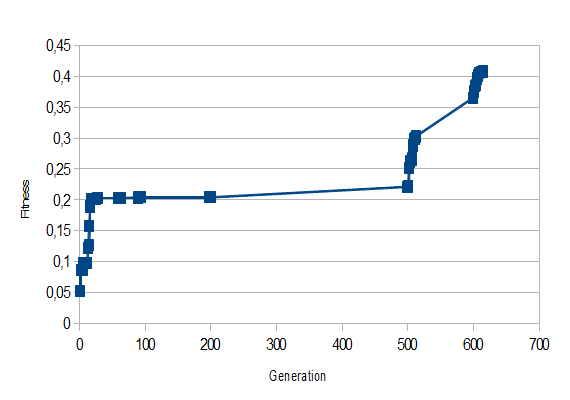
\includegraphics[width=0.5\textwidth]{graphs/fitness5}}\\
	\subfloat[Spike train 3]{\label{fitness8}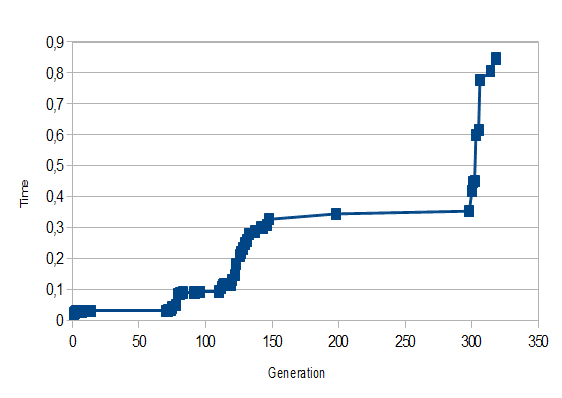
\includegraphics[width=0.5\textwidth]{graphs/fitness8}}
	\subfloat[Spike train 4]{\label{fitness11}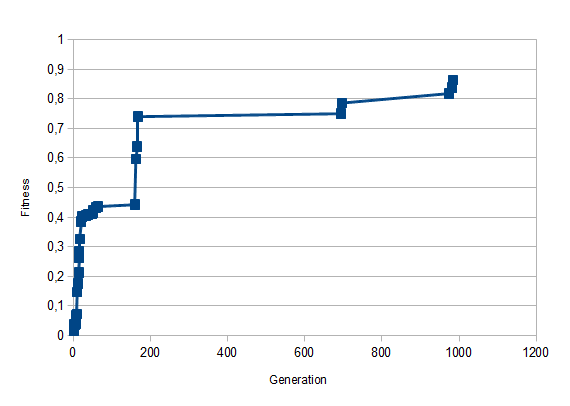
\includegraphics[width=0.5\textwidth]{graphs/fitness11}}
	\caption{This is the fitness graph matching the spike trains developed with Spike Interval Distance Metrics.}
	\label{spikeintervalfitness}
\end{figure}





\begin{figure}
	\centering
	\subfloat[Spike train 1]{\label{activation3}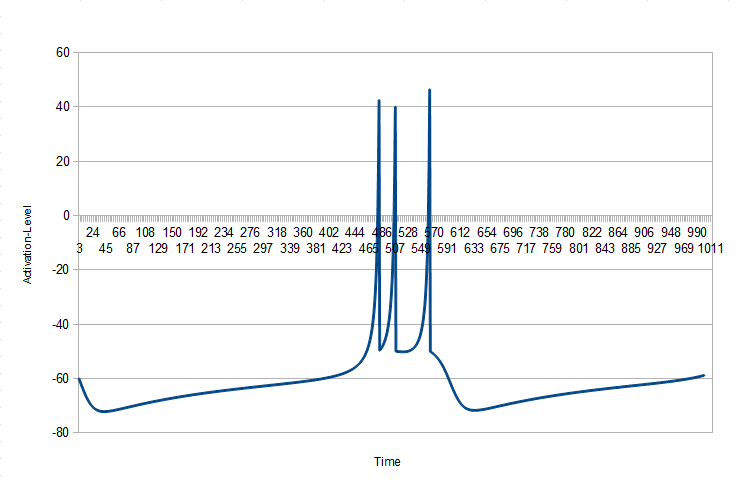
\includegraphics[width=0.5\textwidth]{graphs/activationlevel3}}
	\subfloat[Spike train 2]{\label{activation6}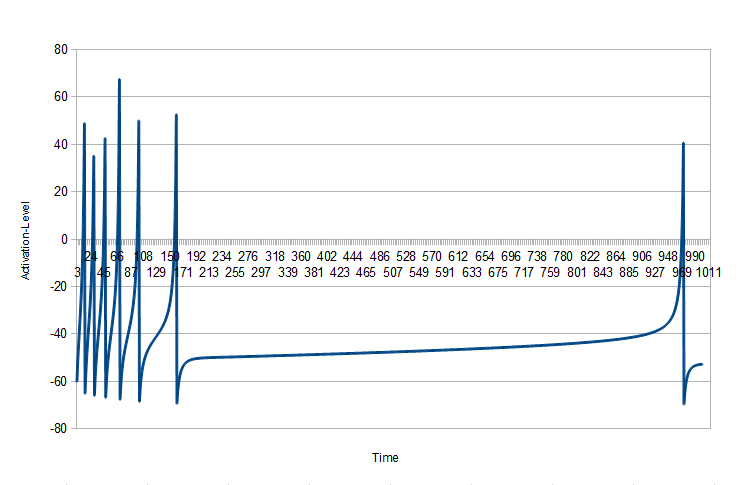
\includegraphics[width=0.5\textwidth]{graphs/activationlevel6}}\\
	\subfloat[Spike train 3]{\label{activation9}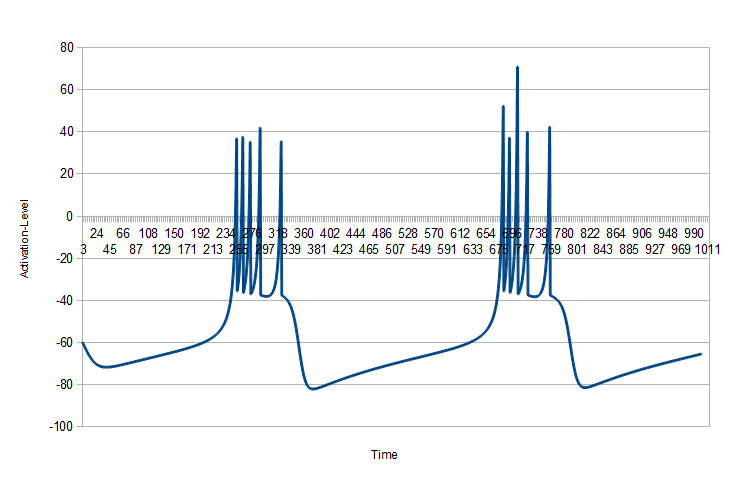
\includegraphics[width=0.5\textwidth]{graphs/activationlevel9}}
	\subfloat[Spike train 4]{\label{activation12}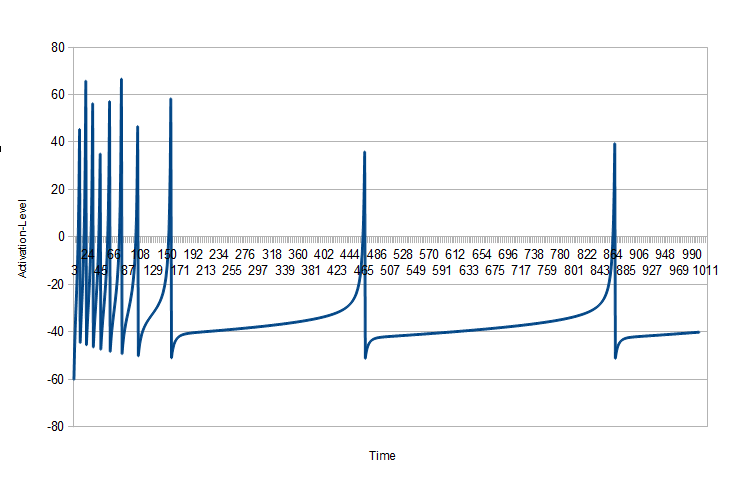
\includegraphics[width=0.5\textwidth]{graphs/activationlevel12}}
	\caption{This is the closest-to-target spike trains developed with Wave Form Distance Metrics.}
	\label{wave}
\end{figure}

\begin{figure}
	\centering
	\subfloat[Spike train 1]{\label{fitness3}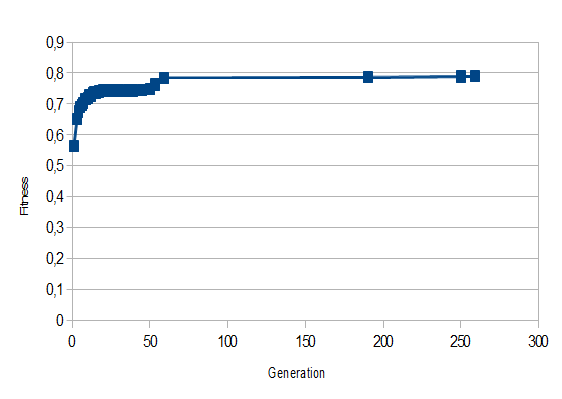
\includegraphics[width=0.5\textwidth]{graphs/fitness3}}
	\subfloat[Spike train 2]{\label{fitness6}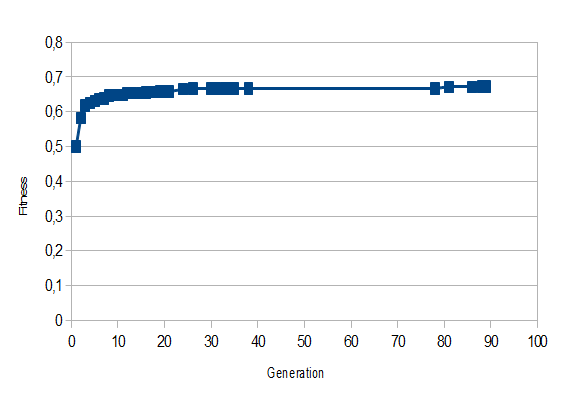
\includegraphics[width=0.5\textwidth]{graphs/fitness6}}\\
	\subfloat[Spike train 3]{\label{fitness9}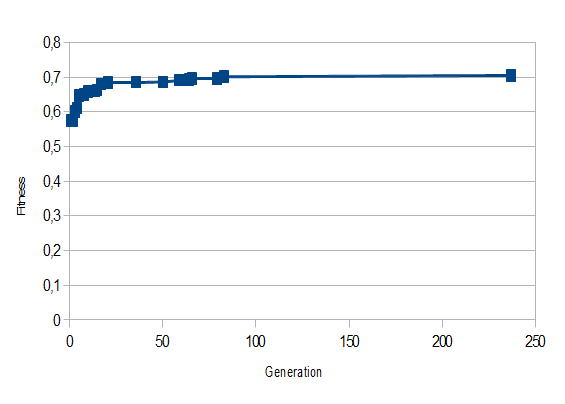
\includegraphics[width=0.5\textwidth]{graphs/fitness9}}
	\subfloat[Spike train 4]{\label{fitness12}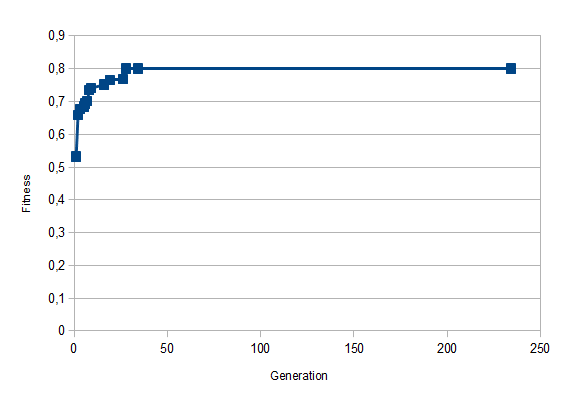
\includegraphics[width=0.5\textwidth]{graphs/fitness12}}
	\caption{This is the fitness graph matching the spike trains developed with Wave Form Distance Metrics.}
	\label{wavefitness}
\end{figure}
\section{Discussion}

\subsection{Mapping}
We have implemented it as a developmental 1-1 mapping between the genotype and phenotype. This is because each 10 bit in the genotypes gives a unique value in the phenotype that acts as a parameter. These are used to create 1001 values that are used for fitness evaluation. No form of normalization or other manipulation is done. As a result any simple mutation or crossover with a different genotype gives a new unique phenotype. 


\subsection{Practical Implications}
The tool tells us about how the neuron works. Which parameters effect it and how it responds to different doses of these. When will it fire spikes and so on. 
A computational neuron scientist could use this to simulate the neuron in different environments. He could use it to try to build small parts of the brain to get a better understanding of the relations of different neurons. 
He could work with the health department to try out new medicine on a early stage to see the effect it could have on the brain.  

\subsection{Other Problem Domains}
Another version of this tool could be used in speech recognition, where the algorithm would evolve to better understand recognize the user. Sound can be seen as waves and could therefore be represented in a similar way, where each letter in the alphabet was represented by X bits and the phenotype is a spike train per letter, where each spike is the most prominent frequency for each sound frame (ref: artificial intelligence project last year). 

The sketch would be similar to the one in Figure 1 in the paper.



\end{document}